\chapter{Emulation Systems}
\label{chap:emulation}

To analyze a system, we must effectively represent its behavior for some case, or set of cases, of interest.
This dissertation is concerned with the emulation of systems or the effective duplication of a system for the purpose of identifying flaws, particularly with respect to security.
In Chapter~\ref{chap:rehost}, we will consider the process of rehosting a system to a different domain in the context of hardware and instruction set emulators, which often allow complex embedded and cyber-physical systems to be analyzed on consumer desktop computers, e.g. laptops, and discuss dynamic analysis, a form of simulation which involves instrumentation of the system under analysis, in this context.
Chapter~\ref{chap:integreat} and Chapter~\ref{chap:info} will discuss consider high-level emulators, copies of a system in a more abstract domain, and function extraction, strategies allowing researchers to dissect complex hardware, firmware, and software systems into testable sub-components.
Both Chapter~\ref{chap:rehost} and Chapter~\ref{chap:rehost} consider the use of symbolic execution and abstract interpretation as a mechanism for emulation, as these techniques explore multiple execution paths and thus implicitly emulate any single, particular execution trace as long as their lifting, semantics, and search strategies are able to identify it.
Every one of these discussed formalisms is well-known and each has several systems that implement the technique or strategy for a variety of real-world use cases~\cite{bellard2005qemu, quynh2015unicorn, deng2013bistro, caballero2009binary, sen2013jalangi, zaddach2014avatar, wang2017angr, cadar2008klee}.
This dissertation may be the first to organize these approaches as forms of emulation---detailed literature reviews are included alongside Chapters~\ref{chap:rehost},\ \ref{chap:info}, and~\ref{chap:integreat}.

In this chapter, we will introduce four different forms of emulation used in the analysis of complex systems.
For each form, we will identify contemporary systems that implement the approach, define its nature and limitations, and provide examples.

\section{Peripheral Emulators and Instruction Set Simulators}
\label{sec:hardemu}

Embedded systems have different requirements than general purpose computers, and typically interact with specialized peripheral devices, such as actuators, and often run on different architectures designed for low power or high reliability usage (though the choice of ISA may also be due to age, cost constraints, and similar root causes).
We next define the core elements of emulators designed to duplicate the operation of embedded systems on general purpose computers~\cite{armstrong2019isa}.

\paragraph{Micro-architectural Semantics}

Base semantics for a micro-architecture consist of the behavior and specification of \emph{instructions} which are capable of being executed, the \emph{state} these instructions can affect, and \emph{peripheral} interfaces, such as memory mapped I/O.
Instructions and state capture of the security model of the architecture, such as exception handling and memory model capabilities (e.g. read-only access).
Peripheral interfaces define the capacity for the microarchitecture to interact with its environment, though not the behavior of the peripherals themselves (discussed in Sec.~\ref{sec:periphs}).
As an example, semantics may refer to the content of the 12,940 pages of the Architecture Reference Manual~\cite{arm2023ref}, which describes the behavior of the ARMv8-A ISA and the representation of the processor's state.
The entire semantics of the micro-architecture is typically captured in a \emph{specification language} for establishing the relationships between components.

Complex micro-architectural semantics may also be established through \emph{microprogramming}.
Microprogramming is a technique for implementing the behavior of an instruction by executing a sequence of simpler instructions.
The execution of several microcode instructions effectively emulates the behavior of a single instruction.
As a result of microprogramming and similar complex semantics, modeling the behavior of a processor is a highly complex task and provides continuous challenge to development of effective simulations for embedded systems.

\paragraph{Instruction Set Simulation}

An instruction set simulator (ISS) simulates the execution of instructions for a given ISA, typically by maintaining the state of the processor in its memory.

There are two primary approaches to implementing an ISS.
The first is to implement the behavior of each instruction in the ISA in a programming language, such as C, and to execute the instructions in the simulator by calling the appropriate function, maintaining the processor state in variables.
The second is to translate the effective behavior of the instructions into equivalent instructions on the host system, and to execute the translated instructions.
The first approach is easier to implement but the second approach is typically faster, as it avoids the overhead of function calls and the need to maintain the processor state in variables.
Modern architectures also increasingly support \emph{virtual machine} (VM) extensions, which allow the host system to adopt the second approach while maintaining security.

For many architectures there exist semantics that do not exist outside of reference documentation and the processor itself.
For these elements, the simulator must either ignore these semantics or emulate them through translation helper routines.
These helper routines and the translation rules for the simulator form an intermediate representation of the target's micro-architectural semantics.
The simulator may then be reused and leveraged to emulate a number of systems that are based on the represented ISA without necessitating ownership of a chip implementing the ISA.

\begin{example}[QEMU]
\end{example}
QEMU is a general purpose emulator that supports a wide variety of ISAs and hardware peripherals~\cite{bellard2005qemu}.
QEMU is both a full system emulator, meaning that it is capable of emulating the behavior of an entire system, including peripherals, and capable of emulating the behavior of a processor in a virtual machine, which allows it to leverage the virtual machine extensions of the host system to accelerate the emulation of the target processor.
In cases where native execution is not possible, QEMU will emulate the instruction by executing a sequence of Tiny Code Generator (TCG) instructions operating over a C struct that stores the target architecture's micro-architectural state.
For example, the following PowerPC instruction:

\begin{center}
\begin{lstlisting}[]
0xfff0010c:  stw    r0,4(r1)
\end{lstlisting}
\end{center}

\noindent
translates into the following TCG instructions (where qemu\_st\_i32 refers to the \emph{guest} memory):

\begin{center}
\begin{lstlisting}[]
0xfff0010c:  movi_i32    tmp1,$0x4
	     add_i32     tmp0,r1,tmp1
	     qemu_st_i32 r0,tmp0,beul,3
\end{lstlisting}

\end{center}

TCG instructions are a RISC-like instruction set that is designed to be easy to translate to the host system's ISA, and serve as an intermediate representation for the emulated system's machine code~\cite{tcg}.
Due to the complexity of certain micro-architectural semantics, QEMU also contains hundreds of TCG helper methods, which operate over the same C structure for the target architecture using C code.
These helper functions are triggered by failures in the translation process, and because not all of them are supported or correct, QEMU serves to emulate targets rather than reproduce them.

Note that the emulation process itself is composed of a larger execution loop, which is responsible for fetching instructions, translating them to TCG instructions, executing them, and modeling the behavior of hardware peripherals and interactions between multiple processors with respect to a given ISA's interfaces.

\paragraph{Hardware Peripherals}
\label{sec:periphs}

A \emph{peripheral} emulator models the behavior of hardware peripherals in order to better emulate the behavior of the overall system.
As a result, hardware peripherals must be represented either by connecting the emulator to the actual hardware, or by reproducing the peripheral in software.
As the space of potential peripherals is theoretically infinite, it becomes more essential to explicate the interfaces by which information is passed from hardware to the emulator.

Hardware peripherals are typically connected to the processor through a \emph{bus}, which is a shared communication channel that allows the processor to communicate with the peripheral.
Interfaces to a given bus are varied and dependent on the specific micro-architecture, as bus is a catch-all term covering hardware, software, and involved protocols.
For example, a processor may communicate with a peripheral through a memory-mapped I/O interface, which allows the peripheral to be accessed through the processor's memory interface, or a peripheral may communicate to the processor via an interrupt controller, which signals an exception to the processor.

A peripheral emulator must emulate the behavior of the peripheral and the behavioral portions of the processor's interface to the bus not covered by the ISS.
This is non-trivial as it can require deducing specific information about the peripheral layout and memory model of the embedded system under analysis, such as the I/O addresses of a given peripheral.
This information is not necessarily available for proprietary embedded systems and in these cases must be inferred from firmware code or other sources.\footnote{For example, Systems-on-Chip (SoCs) may be programmed with specific fuse values and flashed with read-only memory to indicate information about the peripheral model and some modern operating systems use specification files, e.g. device tree blobs, to indicate the layout of memory.}

\paragraph{Instrumentation}

For the purposes of this thesis, we are interested in \emph{instrumentation} of the ISS and peripheral emulator to collect information about the execution of the target system (Tab.~\ref{tab:instruments}).
The amount of instrumentation possible is dependent upon both the technique used to analyze the system and the completeness of the emulation.

Because these emulators have complete insight into the behavior of hardware, it is generally possible to \emph{actively} instrument them in order to collect information about execution.
Each instruction translation can be modified to collect information about various flows of execution, such as transfers of control or data.
It is also possible to inject artificial instructions and data into the emulated system, in order to explore the system's behaviors during certain peripheral interactions or when receiving particular inputs.
Extending this definition, it is also possible to execute the system from an entirely synthetic state in order to model specific behavioral traces.
If the simulator is sufficient, then it is also possible to use active instrumentation to secure otherwise insecure operations, such as by adding bounds checks to memory accesses or by adding checks to ensure that the system is not in an invalid state.

% table of active instrumentation techniques
\begin{table}[h]
\centering
\begin{tabular}{|l|l|}
\hline
\textbf{Technique} & \textbf{Description} \\ \hline
\multirow{2}{*}{Instruction Injection} & \multirow{2}{*}{Modifies the translation of or injects instructions} \\
 & \\ \hline
\multirow{2}{*}{Data Injection} & \multirow{2}{*}{Introduces data into the system at some location} \\
 & \\ \hline
\multirow{2}{*}{Synthetic Execution} & \multirow{2}{*}{Executes the system from a synthetic state} \\
 & \\ \hline
\multirow{2}{*}{Secure Policy Enforcement} & \multirow{2}{*}{Adds security checks to the emulated system} \\
 & \\ \hline
\multirow{2}{*}{Monitoring Frameworks} & \multirow{2}{*}{Monitors the execution trace of the emulated system} \\
 & \\ \hline
\multirow{2}{*}{Interface as Subsystem} & \multirow{2}{*}{Incorporates the emulator into a larger system} \\
 & \\ \hline
\end{tabular}
\caption{Active and passive instrumentation in instruction set and peripheral emulators.}
\label{tab:instruments}
\end{table}

\emph{Passive} instrumentation is also possible, and active techniques are often combined with passive techniques to improve analysis.
This involves implementing monitoring frameworks which operate on the execution trace of the system and temporal reasoning operations for interpreting this trace.
These frameworks can provide performance bench-marking information but also significantly aid in the reverse engineering of the target system by indicating key information, such as explored paths in a symbol-stripped binary.
Passive instrumentation may also use the emulator as a black box and incorporating it into a larger system such as an environmental simulator, to evaluate the dynamics of the larger system.

\section{Dynamic Analysis}
\label{sec:dynanal}

Instrumentation is one method of \emph{dynamic analysis}, which analyzes the behavior of a system or emulation during execution.
To be concrete, the system must be running for it to be considered dynamic, and the analysis must be performed during execution, and the forms used for this dissertation include live binary rewriting, fuzzing, the use of debugger, and passive monitoring.

\paragraph{Live Binary Rewriting} Sometimes it is possible to add self-modifying instructions to a binary in order to change its behavior as it executes.
For a given system, different forms of rewriting and instrumentation are possible, and most include the use of \emph{shim} code injected between the operations of other code for instrumenting the state of the system.
The shim itself can be implemented in a variety of ways, such as by using a \emph{trampoline} which maintains the setup and tear-down of the shim's state during instrumentation.

As a common example, the length of a call instruction on i386 (x86) is a 5-byte instruction, consisting of one byte for the opcode and four bytes for the address of the function to call.
As long as the four byte offset is sufficiently small, the actual call target location information only requires the middle three bytes of the instruction.
In these cases, these three bytes can be shifted over by one, and the call instruction may be modified to a 2-byte interrupt instruction, which transfers control to an interrupt based trampoline for the performance of instrumentation and, reads the remaining three bytes to determine the correct return address, and then self-modifies the shim to replicate the control transfer using the three byte offset (Fig~\ref{fig:livebinaryrewriting}).
This same technique was used to develop exploits for the CMU-900 in Chapter~\ref{chap:rehost}.

% tikz figure depicting the above instrumentation (instruction rewriting) technique
\begin{figure}[h]
\centering
\begin{tikzpicture}[node distance=0.5cm]
	% two halves, one labeled "before instrumentation" and the other "after instrumentation"
	% the left will have "\texttt{call \_func} [0xE8, 0x12, 0x34, 0xFF, 0xFF]", with the last 0xFF highlighted in red and labeled "unneeded". On the right we have "\texttt{int 0x3} [0xCD, 0x03, 0x12, 0x34, 0xFF]"
	\node[draw, minimum width=4cm, text width=8cm, align=center] (before) {\texttt{call \_func:		0xE8, \textcolor{blue}{0x12, 0x34, 0xFF,} \textcolor{red}{0xFF}}};
	\node[draw, minimum width=4cm, text width=8cm, align=center, below=1cm of before] (after) {\texttt{int 0x3:		0xCD, 0x03, \textcolor{blue}{0x12, 0x34, 0xFF}}};
	% arrow with a label "shim injection" between the two halves
	\draw[->, very thick] (before) -- node[right] {Shim Injection} (after);
\end{tikzpicture}
\caption{Example of binary rewriting.}
\label{fig:livebinaryrewriting}
\end{figure}

\paragraph{Fuzzing} Fuzzing is a technique for generating inputs to a system in order to explore its behavior.
In general, fuzzing must be performed on an emulation rather than the system itself, as it is necessary to reset a correct initial state for fuzzing, and many crashes or unexplored behaviors may damage the real system.
For the discovery of bugs, fuzzing is effectively an intelligent dictionary attack which must infer the right inputs to test from a large number (potentially exponential) of possible inputs.
Effective fuzzing also requires careful definitions of \emph{exit conditions}, which indicate when a given input has not found any interesting path, as exploring paths which ``hang'' decreases overall analysis performance.
The most common fuzzers in use today are variations of American Fuzzy Lop (AFL)~\cite{zalewski2017technical}, which provides a general framework and API for building more advanced fuzzers attached to emulators.

\paragraph{Debugging} Debuggers are a common tool for analyzing the behavior of a system, and are often used in conjunction with other techniques.
Similar to a shim, debuggers work by halting the execution of a system at a given point, allowing the user to inspect or modify the system's state, and then resuming execution.
These inspection routines may also be automated, and can be used to collect information about the system's state during execution, similar to instrumentation.
For this purpose, many emulators, like QEMU, include a debugging (gdb) server which allows the analyst to connect to the emulator and inspect the system using common mechanisms, e.g. reading memory values.

\section{High Level Emulators}
\label{sec:highlevel}

While the above techniques are often necessary for the analysis of opaque embedded systems with symbol-stripped firmware, in many cases binaries also originate from standard consumer hardware.
For these binaries \emph{functional} or \emph{high level} emulation (HLE) is appropriate---emulation that does not require the rehosting of system components, and directly operates on program representations.
Standard executables like Microsoft Word are distributed as a binary in a common format with some symbols intact, and emulation can run on standard laptop hardware as the system does not need significant rehosting.
These binaries can be instrumented, translated, or analyzed using a number of tools, including symbolic reasoning frameworks and standard tools from formal methods.
However, these emulators can also be generated using \emph{function extraction}, \emph{summarization}, and \emph{decompilation} of embedded system binaries.

A HLE can make the model of the system more effective and useful while sacrificing authenticity.
These emulators abstract the lower level components or software of the system either by assuming they are already present on the host or by ignoring them altogether.
One benefit of this approach is that it can more easily address high-level correctness concerns, such as the reachability of certain system states, as it does not require a thorough analysis of the system's sub-components and semantics.
This approach is also independent of detailed hardware specifications but is less flexible, as the high-level emulator defines a limited API for the analysis of the system under consideration.
Moreover, a given high-level emulator will be standardized to a particular interpretive domain, e.g. a dynamical or hybrid system interpretation, and does not simulate the behavior of the system under study, which may be possible to model using mathematics but is only exactly specified by the system's implementation in itself.

As more complex, widely used systems and software become prevalent, HLEs become critical.
Supporting the semantics of each detail for a complex system is often infeasible or simply wasteful, as the features are already present on the host for the emulation or not necessary for the analyst's goals.
Low-level emulations are also becoming easier to generate as systems move to single, well-understood architectures like ARM.

\paragraph{Function Extraction}
HLEs often involve some method of \emph{function extraction} for a given component from a complex system, which allows a portion of the system to be emulated in isolation from other components.
Extraction can involve a range of techniques, including program slicing, abstract interpretation, lifting and \emph{summarization}.
A summarization of a function $f$ is given by the following definition~\cite{interpolation}:

\begin{definition}[Function Summarization]
\label{def:summarization}
Let $f$ be a function, $v$ a bound on the number of unrolled loops and recursive calls, $R_{v}^{f}$ a set of tuples of computations in $f$ over $v$, $\mathbb{D}$ a domain function mapping from inputs to outputs of $f$, then $S$ s.t. $R_{v}^{f} \subseteq S \subseteq \mathbb{D}$ is a summary of $f$.
\end{definition}

This definition in itself is limiting as it only considers a strict subset of the map from the inputs to the outputs of the computation $f$, and does not consider the relations that exist between tuples in $R_{v}^{f}$.
Thus it becomes appropriate to consider a more general definition of \emph{logical translation}, which uses propositions to extract system components.

\begin{definition}[Logical Translation]
\label{def:nested-summarization}
	Let $f$ and $f'$ be functions, $P = p_{1}, p_{2}, \dots $ possible
	execution paths through $f$, $\Phi = \phi_{1} . \phi_{2} . \dots
	\phi_{n}$ a set of statements in natural deduction for resolving the
	relationships between symbols in one computational domain function,
	$\mathbb{D}$, mapping from inputs to outputs of $f$, to another domain
	function, $\mathbb{D}'$, mapping from inputs to outputs of $f'$,
	$A_{\Phi(P)}^{f}$ a set of tuples of computations resulting from the
	application of $\Phi$ to $f$ over $P$, then $S$ s.t. $A_{\Phi(P)}^{f}
	\subseteq S \subseteq \mathbb{D}'$ is a logical translation of
	$p$.
\end{definition}

Often the specific translation process is not fully proven for real-world systems and instead adopts \emph{heuristics} or short-cuts which are assumed to be correct in most cases.
An example application of logical translation in this dissertation is the extraction of glyph positioning schemes from PDF document creation software by deducing the C representation of important computations from data-flow analysis (dynamic instrumentation) of machine code operations.

Regardless of the method used, the resulting extracted function may be used as an emulator to verify and understand the behavior of the system, but may be missing non-extracted interfaces.
There are several methods of addressing this, such as replacing these interfaces with logical summaries, as in the HiFrog~\cite{hifrog} and later UpProver~\cite{upprover} systems, or through the use of fuzzing.
Not extracting hardware peripheral semantics also makes firmware rehosting systems like P\textsuperscript{2}IM~\cite{p2im2020} implicit forms of function extraction of software from a hardware-software system, as evidenced by recent work on incomplete information in firmware specifications~\cite{zhou2022your}.

\paragraph{Environmental Modeling and Communication Channels}

Emulation can extend to the modeling of the \emph{environment} of a system, and oftentimes the extracted function of a single component may not be sufficient to understand the overall real-world behavior or security of a system.
Similar to peripheral modeling, some information about the system's environment may not even be available without additional external analysis.
Non-computational environmental modeling is constrained to three forms of specification, captured by common tool-kits like Matlab Simulink, used in this dissertation: equations, random variables, and logic.
Models of computation and stateful systems in the environment are also possible and captured by the subdomain of \emph{hybrid systems} which unify discrete and continuous state transitions~\cite{henzinger1996theory}.

% screenshots of matlab, example of simulink model
\begin{figure}
\centering
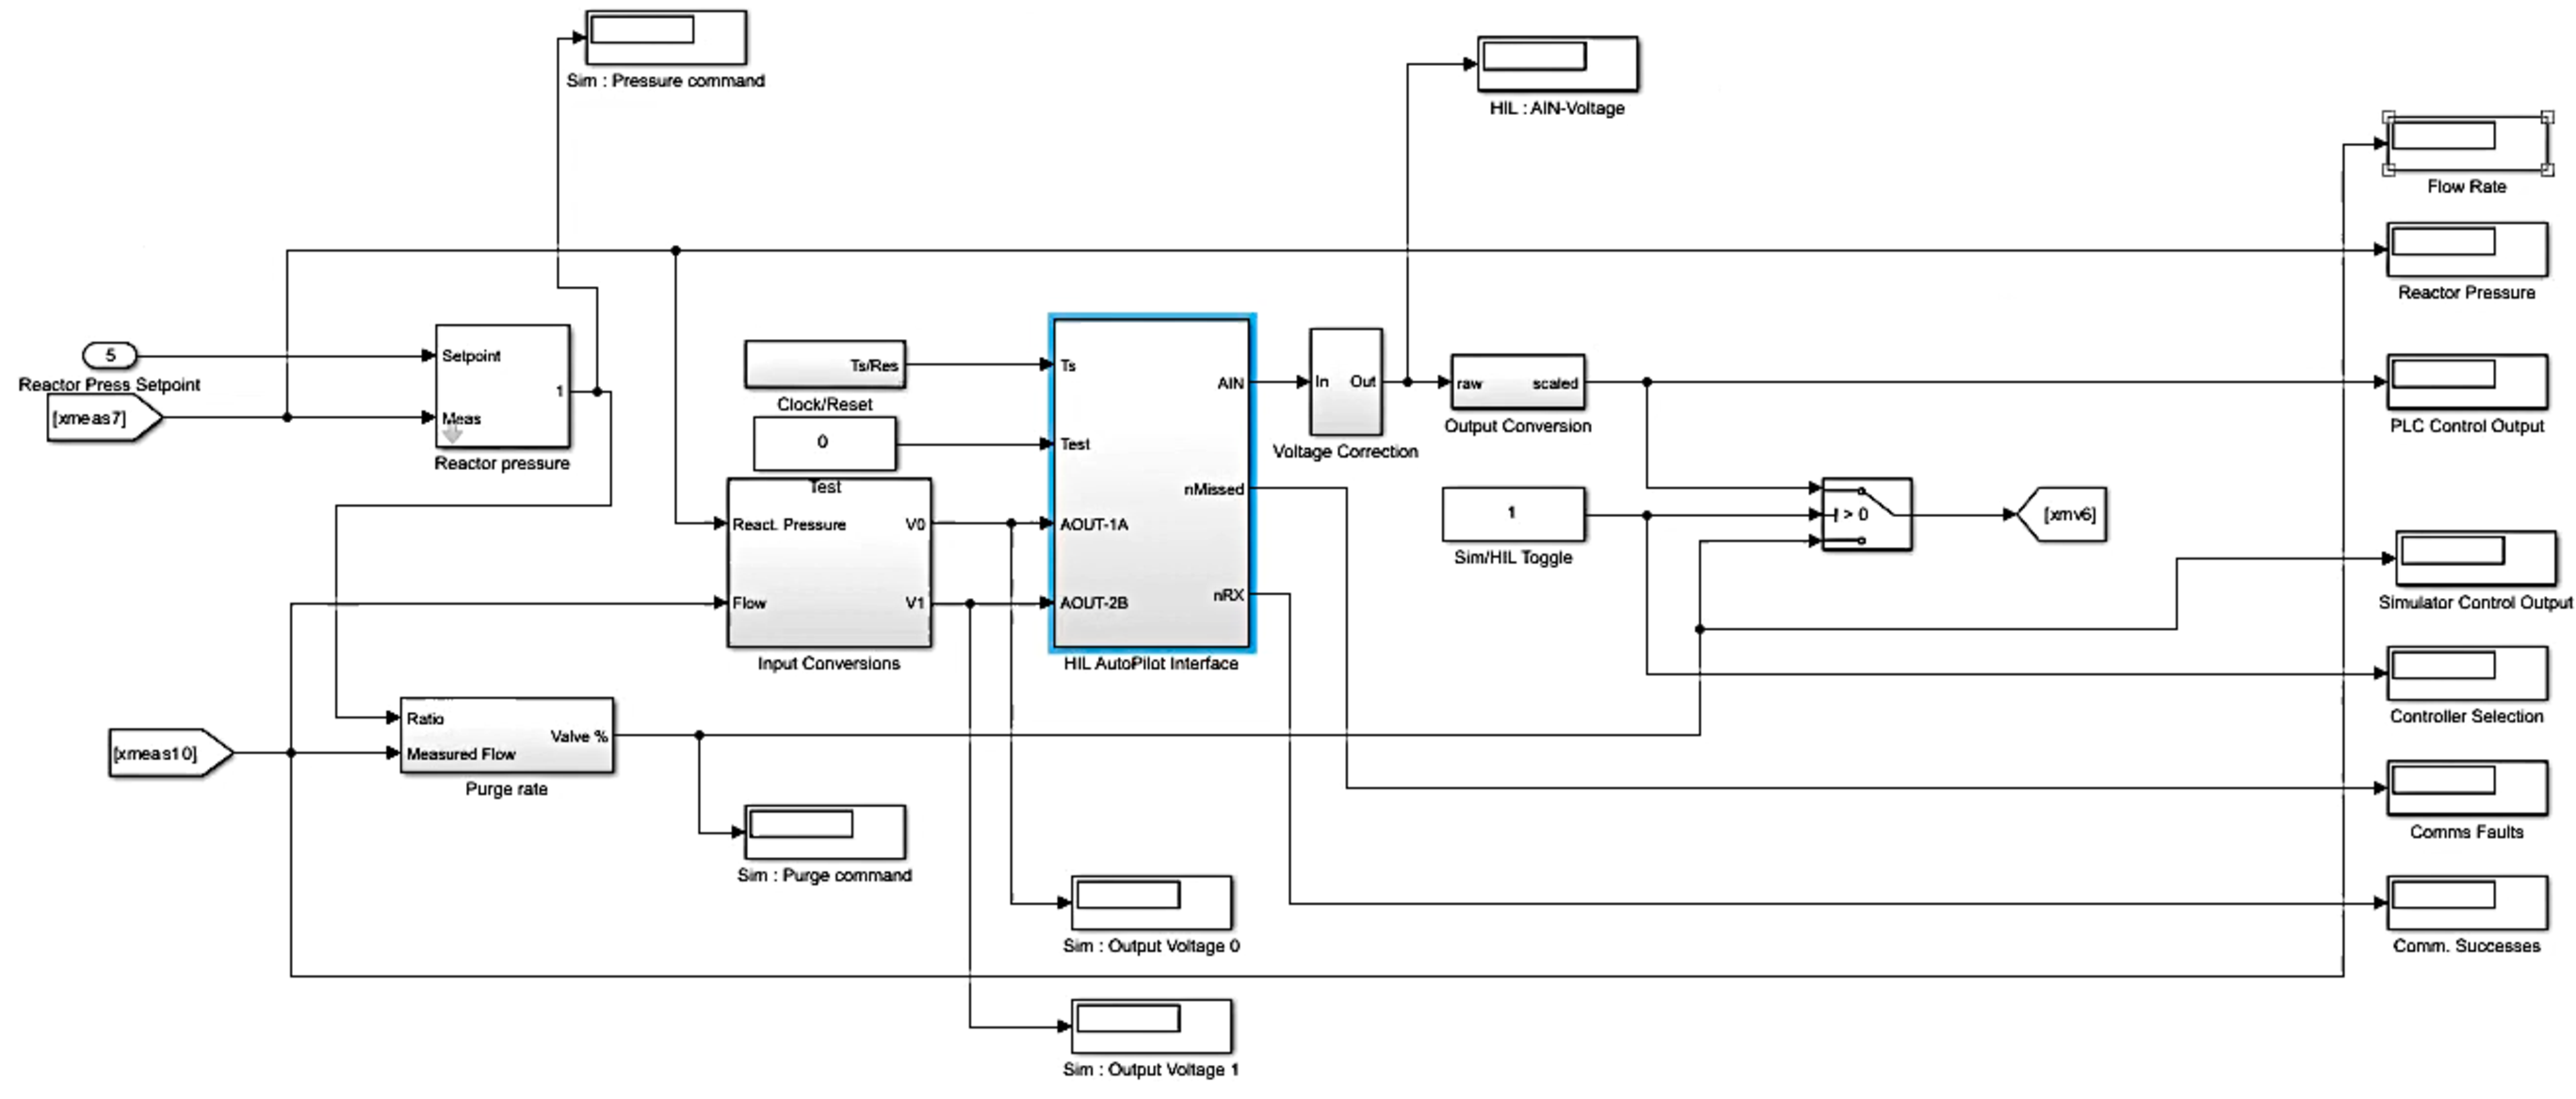
\includegraphics[width=\textwidth]{envir-model.pdf}
\caption{Environmental model emulation inputs and outputs for a chemical plant communicating to a physical Programmable Logic Controller (the blue block) in Simulink.}
\label{fig:envir-model}
\end{figure}

Figure~\ref{fig:envir-model} depicts part of the environmental model for a Tenessee Eastman chemical plant used in this dissertation.
Regardless of the interconnections and components present in a given model, it is notable that the emulation of a given sub-component is entirely determined on what the environmental model can \emph{communicate} to the sub-component.
This concept generalizes across emulation and information theory, captured in by the concept of a \emph{channel}, which consists of an \emph{information source}, \emph{transmitter}, \emph{noise source}, \emph{receiver}, and \emph{destination}~\cite{shannon1948mathematical}:

% tikz drawing of shannon's communication system
\begin{center}
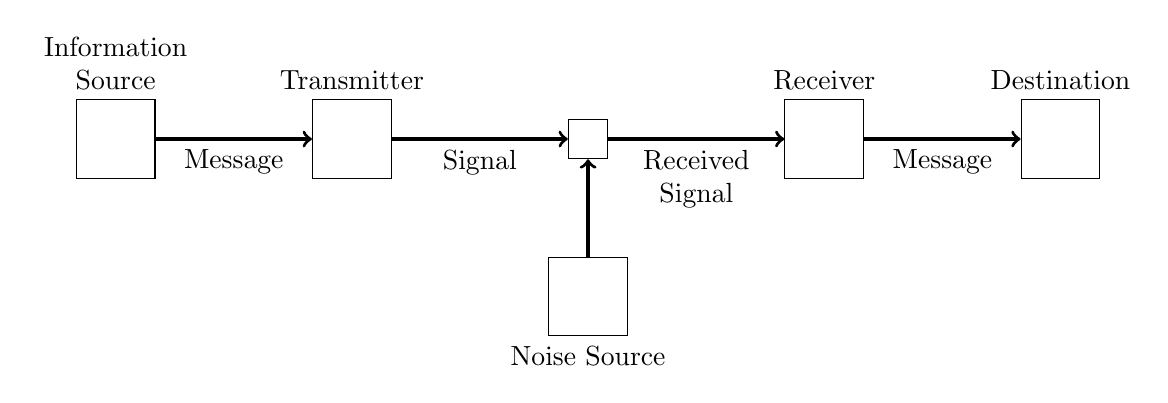
\begin{tikzpicture}
% wrap the text for information source onto two lines
	\node[draw,minimum width=1cm,minimum height=1cm] (source) at (0,0) {};
	\node[draw,minimum width=1cm,minimum height=1cm] (transmitter) at (3,0) {};
\node[draw,minimum width=0.5cm,minimum height=0.5cm] (noise) at (6,0) {};
	\node[draw,minimum width=1cm,minimum height=1cm] (noisesource) at (6,-2) {};
	\node[draw,minimum width=1cm,minimum height=1cm] (receiver) at (9,0) {};
	\node[draw,minimum width=1cm,minimum height=1cm] (destination) at (12,0) {};

% add labels
\node[above, text width=2cm, align=center] at (source.north) {Information Source};
\node[above] at (transmitter.north) {Transmitter};
\node[below] at (noisesource.south) {Noise Source};
\node[above] at (receiver.north) {Receiver};
\node[above] at (destination.north) {Destination};

% message arrow
\draw[->, very thick] (source) -- (transmitter) node[midway,below, align=center] {Message};
% signal arrow
\draw[->, very thick] (transmitter) -- (noise) node[midway,below, align=center] {Signal};
% received signal arrow
\draw[->, very thick] (noise) -- (receiver) node[midway,below, text width=2cm, align=center] {Received Signal};
% message arrow
\draw[->, very thick] (receiver) -- (destination) node[midway,below, align=center] {Message};
\draw[->, very thick] (noisesource) -- (noise) node[midway,right, align=center] {};
\end{tikzpicture}
\end{center}

\noindent
Noise constitutes any distortion of the signal (e.g. loss of information).
The \emph{channel capacity} is the maximum amount of information that can be sent through the channel, and is given by the following equation:

\begin{equation}
C = \max_{p(x)} I(X;Y)
\end{equation}

\noindent
where $p(x)$ is the probability of a given input $x$ to the channel, and $I(X;Y)$ is the \emph{mutual information} between the input $X$ and the output $Y$ of the channel.
Mutual information is defined as:

\begin{equation}
I(X;Y) = \sum_{y \in Y} \sum_{x \in X} p(x,y) \log \frac{p(x,y)}{p(x)p(y)}
\end{equation}

\noindent
where $p(x,y)$ is the joint probability of $x$ and $y$ occurring, and $p(x)$ and $p(y)$ are the marginal probabilities of $x$ and $y$ occurring.
A channel is considered to be \emph{lossless} if the mutual information between the input and output is equal to the entropy of the input, and \emph{lossy} otherwise.
We relate this measure of mutual information to the capacity for an emulation to determine unknown qualities of a system in Chapter~\ref{chap:info}.
Shannon's information channel is often also generalized into an \emph{information flow} which moves between different privilege domains and quantifies security~\cite{sabelfeld2003language, lowe2002quantifying}.

\section{Encoding, Decoding, and Modeling}
\label{sec:encdec}

The formalization of \emph{codes}, systems of rules for the conversion of information, can unify many challenges presented by hardware emulators of Section~\ref{sec:hardemu}, dynamic analysis of Section~\ref{sec:dynanal}, and high level emulation of Section~\ref{sec:highlevel}.
Traditional coding theory is concerned with the design of codes that can be used for the reliable and efficient transmission of information across a noisy channel~\cite{van1971coding, richardson2008modern, bierbrauer2016introduction}.
Standard analyses of codes involve the removal of redundancies and detection of errors and a study of communication channels.
One can also understand emulation as a decoding of a communicated information about the system and an encoding of the system's behavior.
Thus, the efficacy of an emulation is determined by its ability to decode the original system and its ability to encode relevant information, typically thought of as a minimum description length (MDL) or Kolmogorov Complexity.

\begin{definition}[Minimum Description Length]
The length C(s) of the shortest binary string $s$ that is delimited by special marks and that can compute x on the Universal Turing Machine and then halt.
\end{definition}

\noindent
This definition has several limitations:
\begin{enumerate}
	\item It is not computable~\cite{cover1999elements}. Informally, to determine an
		MDL we must execute every program and collect all that stop and
		compute x, choosing the one that has the smallest size.
		However, from the halting problem, we cannot decide if a
		program stops or not. 
	\item There are many programs that compute x and halt, and emulation is
		not strictly concerned with the computation of an
		\emph{optimal} encoding, but an effective encoding in a
		high-dimensional space.
	\item The definition does not provide insight into noise present in the
		channel, and information loss is common in the analysis of real-world
		systems. Equivalently, it does not provide insight into the encoding protocol
		of the information and representation of the system (assumptions made regarding
		the optimal description).
\end{enumerate}

Despite a lack of practical utility, MDL presents an important insight in that it suggests the possibility of measuring the \emph{relative} optimality of two different system encodings.
In practice, we determine the value of an emulation by the results of different dynamic analyses, presented in Section~\ref{sec:dynanal}.
There also exist standard encoding methods for system descriptions, encapsulated by prevalent static analysis techniques, such as taint tracking.

\emph{Taint tracking} is one such standard method of system description, used to encode the flow of information.
For every bit of information in a system, a bit of taint is associated with it, and set to 1 if the information is tainted, and 0 otherwise.
Then, for every operation in the system, the taint of the output is determined by the taint of the inputs and the operation.
If input bits are tainted and these bits decide some bits output, then these output bits will tainted.
The resulting output bits encode how certain bits of information are used throughout the system.
In Chapter~\ref{chap:rehost}, we will use taint tracking to bootstrap the operation of a symbolic execution engine within an instruction set simulator.

For general function extraction, a standard encoding method for a system's operation is an \emph{execution trace}, which can be recorded and then ``replayed'' to emulate the behavior of a system with the possibility of \emph{time-travel debugging}, a form of source-to-sink information-flow analysis capable of extracting the specific operations used to derive a variable.\footnote{
	We scripted the Windows debugger time-travel debugging feature~\cite{timetravel} in order to perform function extraction on the glyph positioning models for the purposes of breaking redactions in Chapter~\ref{chap:info}.}
Execution traces are written by some \emph{interpretation} of the system given by the emulator, a transformation of information which provides that information with a concrete meaning in some context.
A given trace will be incorrect if the emulator does not capture the semantics of the system which are captured by a ``correct interpretation'', e.g. execution on the target micro-architecture, in the trace's output encoding (Section~\ref{sec:hardemu}).

\emph{Modeling} a system is the generation translation of the system's original encoding which is still executable either in the original context or in an emulator.
Formally, a model of a system will preserve some property of the system, such as its behavior or its structure, to some degree of error $\epsilon$.
Given appropriate assumptions on the intended semantics of the system hold, the \emph{correctness} of a model may be determined by a proof demonstrating the outputs of the model are within $\epsilon$ of the outputs of the original system.
This problem is also referred to as the \emph{completeness} of an interpretation~\cite{campion2022partial}.

\begin{algorithm}
\caption{Back-propagation}
\label{alg:backprop}
\begin{algorithmic}[1]
\Procedure{Backprop}{$\mathbf{X}, \mathbf{Y}, \mathbf{W}$}
\For {$l \gets L - 1$ to $1$} % add a comment that this is each layer
\Comment{Each layer}
	\For {$i \gets 1$ to $n$}
\Comment{Each neuron}
		\State $\delta_{i}^{l} \gets (\sum_{j \in L_{i}} w_{ij}^{l+1} \delta_{j}^{l+1}) * f'(z_{i}^{l})$
	\EndFor
\EndFor
\EndProcedure
\end{algorithmic}
\end{algorithm}


\begin{figure}
  \begin{lstlisting}
  /* Code ommitted for space */
  else {
    /* Code ommitted for space */
    do {
      pdVar15 = pdVar7 + 1;
      uVar22 = __aeabi_dmul(
        *(undef4 *)pdVar7,
        *(undef4 *)((int)pdVar7 + 4),
        *(undef4 *)(pdVar17 + 1),
        *(undef4 *)((int)pdVar17 + 0xc));
      pdVar17 = pdVar17 + iVar14;
      uVar21 = __aeabi_dadd(
        (int)uVar21,
        (int)((ulonglong)uVar21 >> 0x20),
        (int)uVar22,
        (int)((ulonglong)uVar22 >> 0x20));
      pdVar7 = pdVar15;
    } while (pdVar15 != pdVar11);
  }
  uVar10 = *(undef4 *)(local_78 + 1);
  uVar13 = *(undef4 *)((int)local_78 + 0xc);
  uVar22 = __aeabi_dsub(0,0x3ff00000,uVar10,uVar13);
  uVar22 = __aeabi_dmul(
    (int)uVar22, (int)((ulonglong)uVar22 >> 0x20),
    uVar10, uVar13);
  dVar23 = (double)__aeabi_dmul(
    (int)uVar22, (int)((ulonglong)uVar22 >> 0x20),
    (int)uVar21, (int)((ulonglong)uVar21 >> 0x20));
  /* Code ommitted for space */
\end{lstlisting}
	\caption{Ghidra decompiled code for the sum operation of Algorithm~\ref{alg:backprop}.}
	\label{fig:ann-decomp}
\end{figure}


\begin{example}[Artificial Neural Network]
Consider a system with a sub-component implementing a single back-propagation step of an artificial neural network (ANN), provided in the high-level encoding of Algorithm~\ref{alg:backprop}.
This standard model of the ANN could be ``executed'' by a human reader, but the form of encoding executed by a computer is the low-level encoding of the system, which is a sequence of instructions given in machine code or interpreted from a high-level representation.
Fig.~\ref{fig:ann-decomp}. depicts one such high-level representation, the output of this routine \emph{decompiled} from machine code into a pseudo-C representation by Ghidra using several of the techniques mentioned in this Chapter.
This code, which represents a sub-component of a larger system, could alternatively be modeled by a symbolic executor, such as angr.
Upon reaching a function like \_\_aeabi\_dadd, traditional symbolic execution will enter into the function, interpret it, and return a complex bit-vector operation.

To provide some notion of complexity, one software floating point multiply we studied, for example, had 153 lines of pseudo-C, 116 lines of decompiled assembly, and 15 branches, but a given emulator may interpret only a subset of these instructions.
Extending this notion of emulation to the absolute limit, it is also possible to encode a system in such a manner that \emph{all} internal semantic detail is lost and only the input and output characteristics remain.

We extracted one ARM software floating point value add taken from a real implementation of the above ANN code for a specific compiler and micro-architecture.
Representing this operation as an uninterpreted function, preserving no semantics of the add operation itself, in a format that may be operated on by the Z3 theorem prover~\cite{zthree}\footnote{We split the representation into three assignments for simplicity.} results in the encoding provided in Fig.~\ref{fig:ann-spec}.
The high level of abstraction in this encoding serves as a demonstration for the degree of flexibility possible in symbolic representations of systems.
Thus, the remainder of this dissertation relies on empirical evidence to justify its adopted emulation strategies.

\begin{figure}
  \begin{lstlisting}
tmp = z3.Function('f', [z3.FPSort(11,53)]*3)( z3.fpBVToFP( z3.Concat(r1, r0), z3.FPSort(11, 53)), z3.fpBVToFP( z3.Concat(r3, r2), z3.FPSort(11, 53)))
r0 = z3.Extract(31, 0, z3.fpToIEEEBV(tmp))
r1 = z3.Extract(63, 32, z3.fpToIEEEBV(tmp))
  \end{lstlisting}
	\caption{Example model of a ARM software floating point add as an uninterpreted function.}
  \label{fig:ann-spec}
\end{figure}

\end{example}

